Die \emph{Bauindustrie} ist einer der wichtigsten Sektoren der �sterreichischen Wirtschaft. Einerseits waren im Jahre 2004   rund 21.600 Unternehmen �sterreichs im Bauwesen t�tig (Quelle:~\cite{branchenmonitor}) und andererseits liefert das Bauwesen einen Beitrag von rund sieben Prozent (15,7 Mrd. Euro) zum Bruttoinlandsprodukt.

Au�erdem spielen (�ffentliche) Bauinvestitionen eine gro�e Rolle. Diese stellen eine der effizientesten M�glichkeiten dar, um wachstums- und stabilit�tspolitische Zielsetzungen zu erreichen, indem die Konjunktur \"uber den Multiplikatoreffekt angekurbelt wird\footnote{Vgl. \cite{baujahr}}.

\subsubsection{Bauindustrie}
\label{sec:Bauindustrie}

\begin{figure}
\centering
\caption{Sparten der Bauindustrie, Quelle:~\cite{leitbetriebe}}
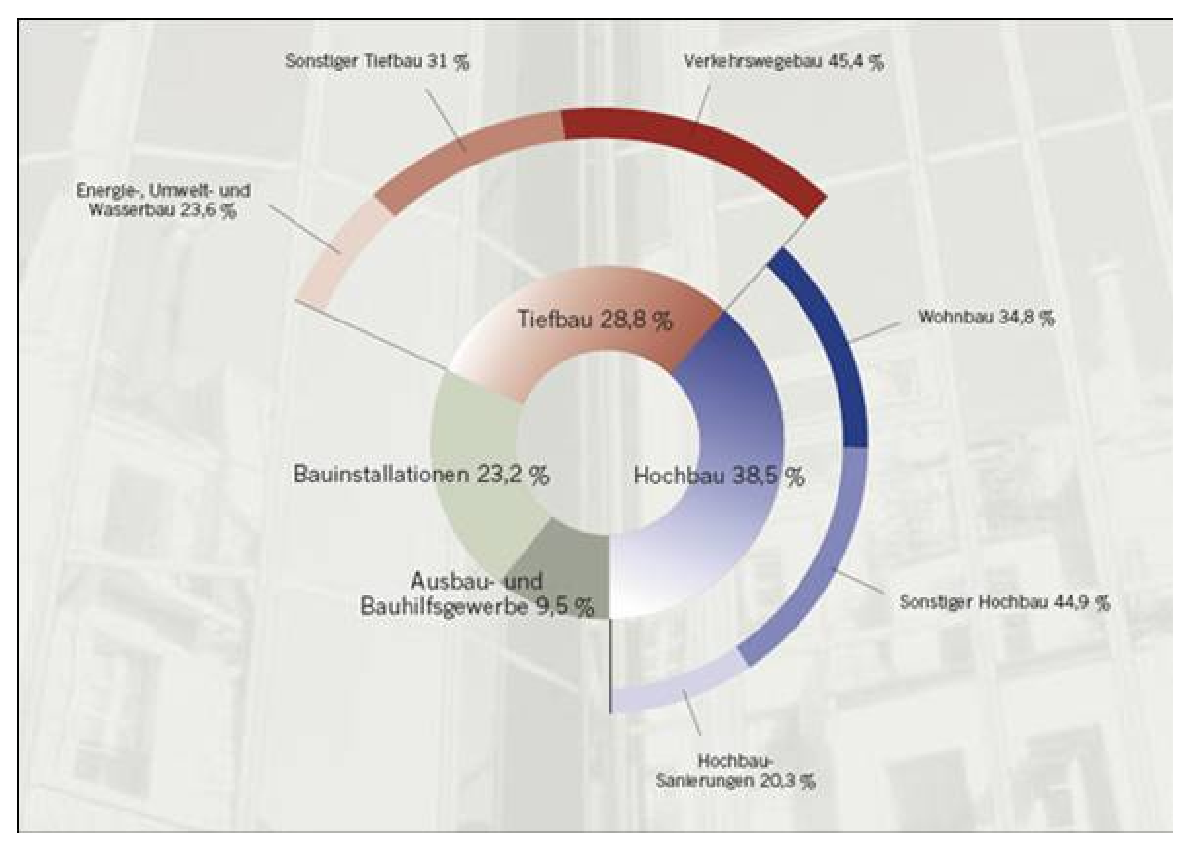
\includegraphics[width = 0.7\textwidth]{branche.eps}
\label{pic:Sparten}
%\cite{www.leitbetriebe.at}
\end{figure}

So beudeutend die Bauindustrie ist, so vielf�ltig sind auch ihre Sparten. Wie in Abbildung \ref{pic:Sparten} ersichtlich, gibt es die Sparten \emph{Hoch- und Tiefbau}, \emph{Ausbau- und Bauhilsgewerbe} sowie die Sparte \emph{Bauinstallationen}, wobei der Hochbau mit einem Produktionswert von \"uber 6 Mrd. Euro den gr��ten Bereich darstellt (Quelle:~\cite{baujahr}).

Nach den schwierigen Jahren 2001 und 2002 und der teilweisen positiven Entwicklung in 2003 und 2004 steigt der Optimismus seit 2005 wieder und es wird mit einem soliden Wachstum gerechnet. Auch die Konjunkturerholung Anfang 2006 wird neben der Sachg\"utererzeugung gr��tenteils der Bauwirtschaft zugeschrieben. Betriebe des Hoch- und Tiefbaus melden aufgrund eines erh�hten Bedarfs an Wohnungen eine g\"unstige Auftragslage, erwarten h�here Preise durchsetzen zu k�nnen und beabsichtigen Personal aufzunehmen. Ebenfalls g\"unstig ist die Auftragslage im Stra�en- und Schienenbau (Quelle:~\cite{AK}), wobei vor allem der Ausbau der Anbindungen an die neuen EU-Mitgliedstaaten ausschlaggebend ist.

\subsubsection{Konjunktur}
\label{sec:Konjunktur}

F\"ur das Jahr 2005 wurde von der \emph{Forschungsgesellschaft f\"ur Bauen, Wohnen und Planen} (FGW) f\"ur die gesamte Bauwirtschaft ein reales Wachstum des Produktionswertes um 1,3~\% prognostiziert. Die tragende St\"utze hierbei ist der Tiefbau mit Zuw�chsen von 4~\%, wohingegen es im Hochbau zur Stagnation kommt. Dies spiegelt sich auch im Baupreisindex nieder: Im Hochbau kam es einer Steigerung der Baukosten, wobei d�e Steigerung der Preise niedriger ausfiel. Dies ist ein Indiz f\"ur den starken Preiswettbewerb im Bauwesen.

Prognosen f\"ur 2006 �hneln den oben beschriebenen Werten. Jedoch konnte mit der Sicherung der Wohnbauf�rderung bis 2008 zumindest eine kleine F�rderung der Sparte Hochbau erzielt werden, daher rechnet das Wirtschaftsforschungsinstitut mit einem Wachstum von 1,4~\%. Tragend bleibt aber der Tiefbau mit einem Wachstum von 2,5~\%. Eine \"Ubersicht \"uber die Prognosen ist in Tabelle~\ref{table:wachstum} ersichtlich. 

Besonders zu betonen ist hierbei, dass vor allem im Bereich des Spezialtiefbaus mit 10 \% f\"ur 2005 ein hohes Wachstumspotential steckt. Im Jahre 2004 betrug das Wachstum in diesem Bereich sogar 25 \%.

\begin{table}
  \centering
  \caption{Bauproduktion nach Sparten, reale Ver�nderung gegen\"uber dem Vorjahr in Prozent (Prognosen 2005 - 2007), Quelle:~\cite{branchenmonitor}}
  \label{table:wachstum}
  \begin{tabular}{|l|r|r c r|}
    \hline
    & FGW && WIFO &\\
    & 2005 & 2005 & 2006 & 2007\\
    \hline
    Hochbau & 0,0 & 0,9 & 1,4 & 1,8\\
    ~~davon:&&&&\\
    ~~Wohnungsbau: & -1,7 & 0,6 & 0,9 & 1,6\\
    ~~Nutzbau: & 1,8 & 1,1 & 2,4 & 2,1\\
    ~~Modernisierung und Sanierung: & -0,8 & - &- &-\\
    Tiefbau &4,0 & 3,2 & 2,5 & 2,7\\
    ~~davon:&&&&\\
    ~~Rohrleitungs-und Kabeltiefbau & -4,1 & - & - &-\\
    ~~Stra�en- und Eisenbahnoberbau & 5,7 & - &- &-\\
    ~~Spezialbau &10,0 & -&-&-\\
    Hoch- und Tiebau gesamt & 1,6 & 1,5 & 1,7 & 2,0\\
    Bauhilfs- und Baunebengewerbe & 0,8 & - &- &-\\
    \hline
  \end{tabular}
\end{table}